%!TEX TS-program = xelatex
%!TEX encoding = UTF-8 Unicode

\documentclass[11pt]{extarticle}
% extarticle is like article but can handle 8pt, 9pt, 10pt, 11pt, 12pt, 14pt, 17pt, and 20pt text

\def \ititle {Joint Action \& the Emergence of Mindreading}
\def \isubtitle {Lecture 2: Minimal Theory of Mind}
\def \iauthor {Stephen A. Butterfill and Ian Apperly}
\def \iemail{s.butterfill@warwick.ac.uk}
\date{}

\input{$HOME/Documents/submissions/preamble_steve_handout}


%itemize bullet should be dash
\renewcommand{\labelitemi}{$-$}

\begin{document}

\begin{multicols}{3}

\setlength\footnotesep{1em}

\bibpunct{}{}{,}{s}{}{,}  %use superscript TICS style bib

\bibliographystyle{newapa} %apalike

%\maketitle
%\tableofcontents






\begin{center}
{\Large
Mindreading \& Joint Action: Philosophical Tools}

Lecture 3: Tracking, Measuring and Representing Beliefs


ButterfillS@ceu.hu
\end{center}

\section{Question}
What could someone represent that would enable her to track, at least within limits, others' perceptions, knowledge states and beliefs including false beliefs? 


\section{Tracking}

%A \emph{mindreading ability} is an ability that exists in part because exercising it brings benefits obtaining which depends on exploiting or influencing facts about others’ mental states.  
%
%An \textit{ability to track} perceptions or beliefs (say) is a mindreading ability which involves exploiting or influencing facts about these states.

%For a subject to \textit{track} the truth of a proposition, $p$, is for the subject's thoughts or actions to nonaccidentally depend in some way on whether $p$.
%%(So that, in principle, one might reliably determined whether $p$ by observing the subject's thoughts and actions.)
%%(And so that, in principle, one could reliably influence the subject's thoughts or actions by determining whether $p$.)
To \textit{track} a subject's belief that $p$ is for your thoughts or actions to nonaccidentally depend in some way on whether this subject believes that $p$.

%To \textit{track} the toxicity of a food item is for your thoughts or actions to nonaccidentally depend in some way on how toxic the food item is.


\section{Automaticity}
A process is \emph{automatic} if whether it occurs is to a significant degree independent of its relevance to the particulars of the subject's motives and aims.
(A process may occur spontaneously without thereby being automatic.)  

Are human adults’ abilities to represent beliefs automatic?
There is evidence for\citep{kovacs_social_2010,Schneider:2011fk} and against.\citep{apperly:2008_back,apperly_why_2010} 

Representing perceptions and beliefs as such---and even merely holding in mind what another believes, where no inference is required---involves a measurable processing cost\citep{apperly:2008_back,apperly:2010_limits}, consumes attention and working memory in fully competent adults,\citealp{Apperly:2009cc, lin:2010_reflexively, McKinnon:2007rr} may require inhibition\citep{bull:2008_role} and makes demands on executive function.\citep{apperly:2004_frontal,samson:2005_seeing}


\section{Minimal theory of mind}
An agent’s \emph{field} is a set of objects related to the agent by proximity, orientation, lighting and other factors.

An agent \emph{encounters} an object just if it is in her field.

A \emph{goal} is an outcome to which one or more actions are, or might be, directed.  (Not to be confused with a \emph{goal-state} , which is an intention or other state of an agent linking an action to a particular goal to which it is directed.)


\textbf{Principle 3}: one can’t goal-directedly act on an object unless one has encountered it.

Application: subordinate chimps retrieve food when a dominant is not informed of its location.\citep{Hare:2001ph}

Application: when observed scrub-jays prefer to cache in shady, distant and occluded locations.\citep{Dally:2004xf,Clayton:2007fh}

An agent \emph{registers} an object at a location [first approximation] just if she most recently encountered the object at that location.

A registration is \emph{correct} just if the object is at the location it is registered at.

\textbf{Principle 4}: correct registration is a condition of successful action.

Applications: 12-month-olds point to inform depending on their informants’ goals and ignorance;\citep{Liszkowski:2008al} chimps retrieve food when a dominant is misinformed about its location;\citep{Hare:2001ph} scrub-jays observed caching food by a competitor later re-cache in private.\citep{Clayton:2007fh,Emery:2007ze}

 
\textbf{Principle 5}: when an agent performs a goal-directed action and the goal specifies an object, the agent will act as if the object were actually in the location she registers it at.

Applications: some false belief tasks \citep{Onishi:2005hm,Southgate:2007js,Buttelmann:2009gy}


\section{Signature limits}
\begin{center}
  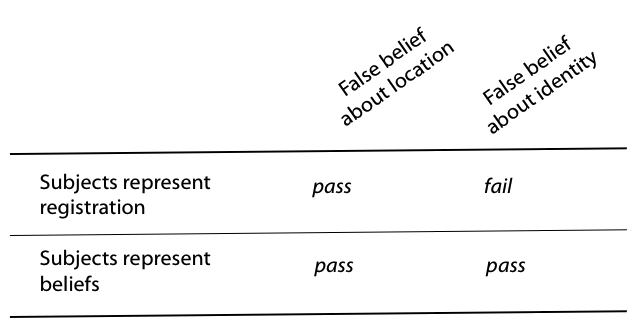
\includegraphics[width=0.3\textwidth]{fig1.png}
\end{center}

\begin{center}
  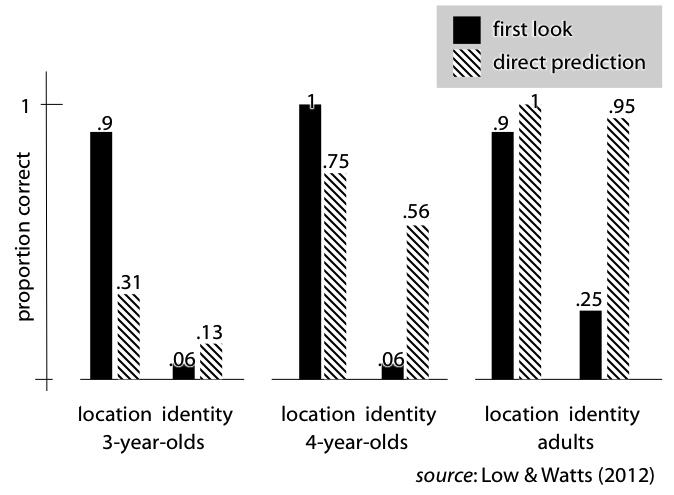
\includegraphics[width=0.3\textwidth]{fig2.png}\citep{low:2010_preschoolers}
\end{center}

\footnotesize 
\bibliography{$HOME/endnote/phd_biblio}

\end{multicols}

\end{document}